\documentclass[a4paper,12pt]{article}
\usepackage{amsmath}
\usepackage{amssymb}
\usepackage{tikz}
\newcommand{\CommaPunct}{\mathpunct{\raisebox{0.5ex}{,}}}
\begin{document}
\title{ECE108 Assignment3} \author{Yi Fan Yu yf3yu@edu.uwaterloo.ca} \date{\today}

\maketitle

\pagenumbering{arabic}
\tableofcontents
\newpage
\renewcommand\thesubsection{\alph{subsection}}
\section{Rolling Dice}
\subsection{Dicerolling1,2,3,4,5,6}
How many times will you always get all six numbers at least one, assuming $n > 6A$ ?
What is the probability of this occurring?\\
\bigskip\\
well let's see the probability of the complement happening, so how many times will I not get all six numbers:\\
Using the inclusion-exclusion principle:\\
  \begin{enumerate}
    \item No 1 :$5^n$
    \item No 2 :$5^n$
    \item No 3 :$5^n$
    \item No 4 :$5^n$
    \item No 5 :$5^n$
    \item No 6 :$5^n$
  \end{enumerate}
  the first set with no 1 seems to have $4^n$ in common with all 5 others\\
  the second set with no 2 seems also to have the same thing\\
  we can see a pattern here... \\
  we remove $6C2(4^n) = 15(4^n)$ to remove all the duplications\\
  then we add $6C3(3^n) = 20 (3^n)$ because we removed too much\\
  then we remove $6C4(2^n) = 15 (2^n)$\\
  then we add $6C5(1^n) = 6$\\
  then we remove $6C6(0) =0$\\
  \bigskip\\
  so we get total occurence of having all 6 numbers is:\\
  \[(6^n) - (6(5^n) -15(4^n) + 20(3^n)- 15(2^n) + 6) \]
  the total probability is then:\\
  \[\frac{(6^n) - (6(5^n) -15(4^n) + 20(3^n)- 15(2^n) + 6)}{6^n} \]
\subsection{DicerollingA,B,C}
How many times will the sum of the number of 1's and 2's equal the
sum of the number of 3's, 4's, 5's and 6's?  What is the probability
of this occurring?
let's say\\
\[ 1 \& 2 \mapsto A\]
\[ 3 \& 4 \mapsto B\]
\[ 5 \& 6 \mapsto C\]
$A \& B \& C$ with all equal possibilities of showing up (1/3)\\
Then we can say we are only throwing a 3-sided dice, therefore the total amount of possibilities while throwing is\\
\[3^n\]
ok for 4 four throws:\\
we could have 2As and 2Bs\\
or 2As,1B and 1C\\
or 2As and 2Cs\\
we can use the fact that $A_{1}$ is indisguishable from $A_{2}$...
and we get 
  \[ \frac{4!}{2!2!} + \frac{4!}{2!} + \frac{4!}{2!2!} \]
  in the first term 2As and 2Bs are indisguishable\\
  in the second term 2As are indisguishable\\
  in the second term 2As and 2Cs are indisguishable\\
  after simplifications...\\
  \[ 2^2 \binom{4}{2} \]
  after writing out it for n = 6
  \[ 2^3 \binom{6}{3} \]
  and for n = 8
  \[ 2^4 \binom{8}{4} \]
  Our final generalized form is:
  \[ 2^{\frac{n}{2}} \binom{n}{\frac{n}{2}} \]
  for 6 sided-dice :

  \[ 2^n 2^{\frac{n}{2}} \binom{n}{\frac{n}{2}} \]
  Our probability is 
  \[ \frac {2^{\frac{n}{2}} \binom{n}{\frac{n}{2}}}{3^n} \]
\subsection{DicerollingA,B,C Part2}
How many times will the sum of the number of 1's and 2's equal the
sum of the number of 3's and 4's and equal the sum of the number of
5's and 6's?  What is the probability of this occurring?\\
Same thing as part I, but now $A$s are indisguishable from $B$s and from $C$s.\\
Even better there is no choice this time, we need the As to equal Bs to equal Cs and the amount of A/B/C = n/3. Never varying\\
Therefore,
  \[\frac{n!}{\frac{n}{3}!\frac{n}{3}!\frac{n}{3}!}\]
For 6-sided:
  \[\frac{2^n * n!}{\frac{n}{3}!\frac{n}{3}!\frac{n}{3}!}\]
  with the total probability at :\\
  \[ \frac {\frac{n!}{\frac{n}{3}!\frac{n}{3}!\frac{n}{3}!}} {3^{n}}\]
\subsection{Rolling 1s}
In how many ways will you roll a "1" at least wtice among all $n$ dice roll s, assuming n>2? What is the probability of this occurring?\\
\bigskip\\
Use the exclusion and inclusion principle
\begin{enumerate}
  \item{size of the set where there is absolutely zero 1: $5^n$}
  \item{size of the set where there is only one 1: $n(5^{n-1})$}
\end{enumerate}
since there is no overlapping,\\
the total occurence is:
\[6^n - 5^n - n(5^{n-1})\]
the probability is then 
\[\frac{6^n - 5^n - n(5^{n-1})}{6^n}\]
\subsection{Rolling 1s generalized...}
In how many ways will you roll a "1" at least $k$ times, assuming $n > k$? 
What is the probability of this occurring?\\
Use the exclusion and inclusion principle
\begin{enumerate}
  \item{size of the set where there is absolutely zero 1: $\binom{n}{0}5^n$}
  \item{size of the set where there is only one 1: $\binom{n}{1}(5^{n-1})$}
  \item{size of the set where there are only 2 1: $\binom{n}{2}(5^{n-2})$} 
  \item{size of the set where there are only k 1: $\binom{n}{k}(5^{n-k})$} 
\end{enumerate}
As we see, there is no overlap between the sets and we can just use sigma nnotation to give the answer.

\[ 6^n - \sum ^k _{i=0} \binom{n}{i}5^{n-i} \]
Probabilities: \\
\[\frac{ 6^n - \sum ^k _{i=0} \binom{n}{i}5^{n-i}} {6^n}\]
\subsection{Communication, actually even more generalization}
You have a communications system that transmits bundles of data
from a source to a destination.  Most bundles are received correctly.
However, there is a random chance of the data in a bundle being in
error.  Roughly every $E^{th}$ bundle is in error.  If you transmit
$n$ bundles, what is the probability of two bundles being
in error?  what is the probability of $k$ bundles being in
error?\\
\bigskip\\
Let's say the bundle is like a E-sided dice, if we roll a 1, we get error
\begin{enumerate}
  \item{size of the set where there is absolutely no error: $\binom{n}{0}(E-1)^n$}
  \item{size of the set where there is only one 1: $\binom{n}{1}((E-1)^{n-1})$}
  \item{size of the set where there are only 2 1: $\binom{n}{2}((E-1)^{n-2})$} 
  \item{...}
  \item{size of the set where there are only k 1: $\binom{n}{k}((E-1)^{n-k})$} 
\end{enumerate}
Probabilities 2 errors: \\
\[\frac{ E^n - \sum ^1 _{i=0} \binom{n}{i}(E-1)^{n-i}} {E^n}\]
\[\implies \frac{ E^n - (E-1)^{n}}{E^n}\]
Probabilities k error: \\
\[\frac{ E^n - \sum ^{k-1} _{i=0} \binom{n}{i}(E-1)^{n-i}} {E^n}\]
\[\frac{ E^n - \sum ^{k-1} _{i=0} \binom{n}{i}(E-1)^{n-i}} {E^n}\]
\pagebreak
\section{Binomial Theorem}
Prove (using induction) the binomial theorem:
\[
(x+a)^n = \sum_{r=0}^n C(n‚ r)x^{n-r}a^r
\]
\subsection{Base Case}
n = 1 case:\\
\[(x+a) = \sum_{r=0}^1 C(n‚ r)x^{n-r}a^r\]
\[(x+a) = \binom{1}{0} x^{1} + \binom{1}{1}  a^1\]
\[(x+a) = x+a \blacksquare \]
\subsection{N+1 Case}
Assuming:
\[
(x+a)^n = \sum_{r=0}^n C(n‚ r)x^{n-r}a^r
\]
Show:
\[(x+a)^{n+1} = \sum_{r=0}^{n+1} C((n+1)‚ r)x^{(n+1)-r}a^r\]
Proof:
\[(x+a)^{n+1} =  (x+a)^n (x+a)\]
\[(x+a)^{n+1} =  \sum_{r=0}^n C(n‚ r)x^{n-r}a^r (x+a)\]
\[(x+a)^{n+1} =  x\sum_{r=0}^n C(n‚ r)x^{n-r}a^r + a\sum_{r=0}^n C(n‚ r)x^{n-r}a^{r}\] 
putting x and a inside of the sigma notation
\[(x+a)^{n+1} =  \sum_{r=0}^n C(n‚ r)x^{n-r+1}a^r + \sum_{r=0}^n C(n‚ r)x^{n-r}a^{r+1}\] 
pulling r = 0 out of the first sum
\[(x+a)^{n+1} =  \binom{n}{0} x^{n+1}+\sum_{r=1}^n C(n‚ r)x^{n-r+1}a^r + \sum_{r=0}^n C(n‚ r)x^{n-r}a^{r+1}\] 
pulling r = n out of the second sum
\[(x+a)^{n+1} =  \binom{n}{0} x^{n+1}+ \sum_{r=1}^n C(n‚ r)x^{n-r+1}a^r + \binom{n}{n}a^{n+1}+\sum_{r=0}^{n-1} C(n‚ r)x^{n-r}a^{r+1}\] 
shifting the second sum forward 
\[(x+a)^{n+1} =  \binom{n}{0} x^{n+1}+\binom{n}{n}a^{n+1}+ \sum_{r=1}^n C(n‚ r)x^{n-r+1}a^r + \sum_{r=1}^{n} C(n‚ r-1)x^{n-r+1}a^{r}\] 
combining the sigmas
\[(x+a)^{n+1} =  \binom{n}{0} x^{n+1}+\binom{n}{n}a^{n+1}+ \sum_{r=1}^n ((C(n‚ r)+C(n,r-1) )x^{n-r+1}a^r\]
\[(x+a)^{n+1} =  \binom{n}{0} x^{n+1}+\binom{n}{n}a^{n+1}+ \sum_{r=1}^n (\frac{n!}{r!(n-r)!}+\frac{n!}{(r-1)!(n-r+1)!} )x^{n-r+1}a^r\]
trying to simply the choose
\[(x+a)^{n+1} =  \binom{n}{0} x^{n+1}+\binom{n}{n}a^{n+1}+ \sum_{r=1}^n (\frac{n!}{r(r-1)!(n-r)!}+\frac{n!}{(r-1)!(n-r+1)(n-r)!} )x^{n-r+1}a^r\]
\[(x+a)^{n+1} =  \binom{n}{0} x^{n+1}+\binom{n}{n}a^{n+1}+ \sum_{r=1}^n (\frac{n!(r+n-r+1)}{r(r-1)!(n-r)!(n-r+1)})x^{n-r+1}a^r\]
\[(x+a)^{n+1} =  \binom{n}{0} x^{n+1}+\binom{n}{n}a^{n+1}+ \sum_{r=1}^n (\frac{n!(n+1)}{r!(n-r+1)!})x^{n-r+1}a^r\]
\[(x+a)^{n+1} =  \binom{n}{0} x^{n+1}+\binom{n}{n}a^{n+1}+ \sum_{r=1}^n \binom{n+1}{r}x^{n-r+1}a^r\]
$\binom{n}{0} = \binom{n+1}{0} = 1$
$\binom{n}{n} = \binom{n+1}{n+1} = 1$
\[(x+a)^{n+1} =  \binom{n+1}{0} x^{n+1}+\binom{n+1}{n}a^{n+1}+ \sum_{r=1}^n \binom{n+1}{r}x^{n-r+1}a^r\]
the two loose terms are the 0th and n+1th terms
\[(x+a)^{n+1} =  \sum_{r=0}^{n+1} \binom{n+1}{r}x^{n+1-r}a^r\]
\[\blacksquare\]
\pagebreak
\section{Graph Questions}

\subsection{a graph with 5 vertices and 3 edges}
yes, any graph can exist with any amount of vertices and edges provided the number of edges are not bigger than the maximum possible amount.\\
for 5 vertices, the maximum amount of edges 
  \[\binom{5}{2} = 10\]
\begin{center}
  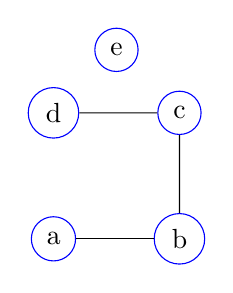
\begin{tikzpicture}
    [scale = .8, auto=center, every node/.style = {circle,draw = blue}]
    \node (n1) at (0,0) {a};
    \node (n2) at (2,0) {b};
    \node (n3) at (2,2) {c};
    \node (n4) at (0,2) {d};
    \node (n5) at (1,3) {e};

    \foreach \from/ \to in {n1/n2,n2/n3,n3/n4}
      \draw (\from) -- (\to);
  \end{tikzpicture}
\end{center}
    
\subsection{a graph with 5 odd-degree vertices with 3 edges}
  it is quite clear that with 3 edges, we are thinking of vertices with
  degree = 1.\\
\begin{center}
  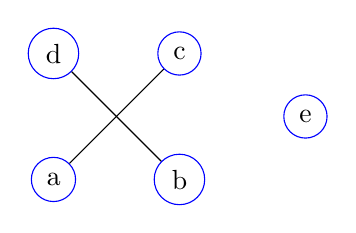
\begin{tikzpicture}
    [scale = .8, auto=center, every node/.style = {circle,draw = blue}]
    \node (n1) at (0,0) {a};
    \node (n2) at (2,0) {b};
    \node (n3) at (2,2) {c};
    \node (n4) at (0,2) {d};
    \node (n5) at (4,1) {e};

    \foreach \from/ \to in {n1/n3,n2/n4}
      \draw (\from) -- (\to);
  \end{tikzpicture}
\end{center}
it is clear that if we try to connect node e, with our remaining 1 edge,
we will create a vertex of degree 2, therefore it is impossible.
\subsection{a connected graph with 5 vertices and 3 edges?}
a connected graph with 4 vertices requires at least 4 edges.
therefore it is impossible to create a connected graph of 5 vertices with only 3 edges...
\begin{center}
  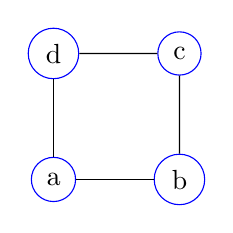
\begin{tikzpicture}
    [scale = .8, auto=center, every node/.style = {circle,draw = blue}]
    \node (n1) at (0,0) {a};
    \node (n2) at (2,0) {b};
    \node (n3) at (2,2) {c};
    \node (n4) at (0,2) {d};
    \foreach \from/ \to in {n1/n2,n2/n3,n3/n4,n4/n1}
      \draw (\from) -- (\to);
  \end{tikzpicture}
\end{center}

\subsection{a directed graph with 5 vertices and 3 edges?}
assuming you mean arcs by edges since in a digraph, there are no edges.

\begin{center}
  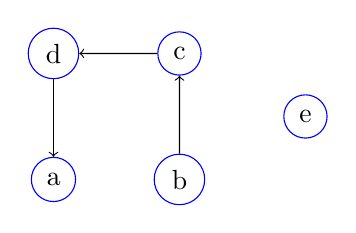
\begin{tikzpicture}
    [scale = .8, auto=center, every node/.style = {circle,draw = blue}]
    \node (n1) at (0,0) {a};
    \node (n2) at (2,0) {b};
    \node (n3) at (2,2) {c};
    \node (n4) at (0,2) {d};
    \node (n5) at (4,1) {e};
    \foreach \from/ \to in {n2/n3,n3/n4,n4/n1}
      \draw[->] (\from) -- (\to);
  \end{tikzpicture}
\end{center}
yes it it possible
\subsection{a disconnected graph (a graph that is not connected) with 5
ices and 7 edges}
no it is not possible, since $K_{4}$ has 6 edges (the maximum amount of edges we can connect with 4 vertices) so we have to connect the 5th node e using our last remaining edge.

\begin{center}
  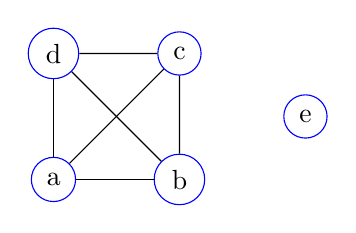
\begin{tikzpicture}
    [scale = .8, auto=center, every node/.style = {circle,draw = blue}]
    \node (n1) at (0,0) {a};
    \node (n2) at (2,0) {b};
    \node (n3) at (2,2) {c};
    \node (n4) at (0,2) {d};
    \node (n5) at (4,1) {e};
    \foreach \from/ \to in {n1/n2,n2/n3,n3/n4,n4/n1,n1/n3,n2/n4}
      \draw (\from) -- (\to);
  \end{tikzpicture}
\end{center}

\subsection{a disconnected, directed graph with 5 vertices and 7 edges }
I assume edges mean arcs (directed edges).
Then yes it is possible since the maximum amount of arcs for $K_{4}$ is 12.\\
So we can completely ignore the 5th node
\begin{center}
  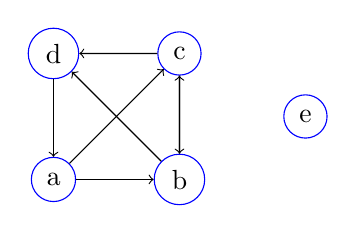
\begin{tikzpicture}
    [scale = .8, auto=center, every node/.style = {circle,draw = blue}]
    \node (n1) at (0,0) {a};
    \node (n2) at (2,0) {b};
    \node (n3) at (2,2) {c};
    \node (n4) at (0,2) {d};
    \node (n5) at (4,1) {e};
    \foreach \from/ \to in {n3/n2,n1/n2,n2/n3,n3/n4,n4/n1,n1/n3,n2/n4}
      \draw[->] (\from) -- (\to);
  \end{tikzpicture}
\end{center}
\subsection{a graph with 3 vertices and 5 edges }
No, since $K_{3}$ has 3 edges and the maximum amount of edges for 3 vertices
is represented by 
  \[ E(K_{3}) = 3\]
\begin{center}
  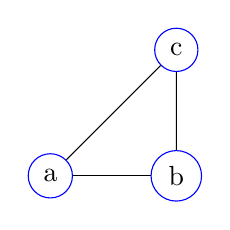
\begin{tikzpicture}
    [scale = .8, auto=center, every node/.style = {circle,draw = blue}]
    \node (n1) at (0,0) {a};
    \node (n2) at (2,0) {b};
    \node (n3) at (2,2) {c};
    \foreach \from/ \to in {n1/n2,n2/n3,n1/n3}
      \draw (\from) -- (\to);
  \end{tikzpicture}
\end{center}
we can't fit 5 edges between 3 vertices.
\subsection{a directed graph with 3 vertices and 5 edges}
I assume that by edges, we are meaning arcs.
then yes it is possible since the maximum amount of arcs for 3 vertices is 6
\begin{center}
  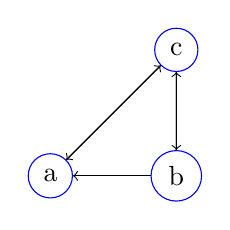
\begin{tikzpicture}
    [scale = .8, auto=center, every node/.style = {circle,draw = blue}]
    \node (n1) at (0,0) {a};
    \node (n2) at (2,0) {b};
    \node (n3) at (2,2) {c};
    \foreach \from/ \to in {n2/n3,n1/n3,n2/n1,n3/n2,n3/n1}
      \draw[->] (\from) -- (\to);
  \end{tikzpicture}
\end{center}

\section{Given a Graph} Given the following graph:

\begin{center}
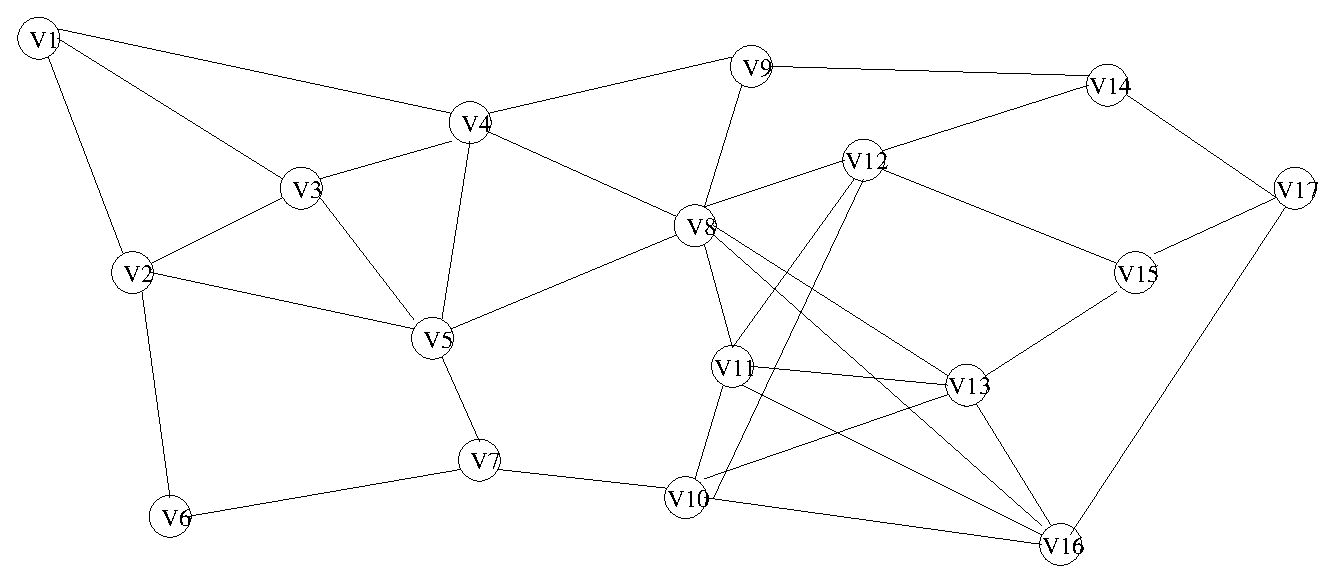
\includegraphics[scale=0.7]{graph.eps}
\end{center}

\subsection{Is this graph connected?}
Yes it is complete, since I can go from any node to any other node.
\subsection{Is this graph complete?  Why/Why not?}
No, there is no edge between V1 and V6.\\
However, there exists a subgraph $K_{4}$
\subsection{What is the minimum degree of the graph?}
minimum degree is 2, on node V6
\subsection{What is the maximum degree of the graph?}
maximum degree is 7, on node V8
\subsection{What is the largest clique in the graph?}
It is a $K_{4}$\\
Here is one of the 2 K4
\[K_{4}\] \[V8,V11,V16,V13\]

\subsection{Is the graph planar? Why/Why not?}
No, there exists a subgraph $K_{3,3}$ $V10,V11,V8,V12,V13,V16$ inside.\\
We know that $K_{3,3}$ is non-planar.\\
\subsection{What is the shortest path from V1 to V17? How long is it?}

\[V1\rightarrow V4\rightarrow V8\rightarrow V16\rightarrow V17\]
it is length 4
\subsection{What is the longest path from V1 to V17?  How long is it?}
\[V1\rightarrow V4 \rightarrow V9 \rightarrow V14 \rightarrow V12 \rightarrow\]
\[V15 \rightarrow V13 \rightarrow V10 \rightarrow V7 \rightarrow\]
\[V6 \rightarrow V2\rightarrow V3\rightarrow V5 \rightarrow\]
\[V8 \rightarrow V11\rightarrow V16\rightarrow V17 \]
length of 16. All the vertices are visited exactly once
\end{document}
